\باب{امکانیات اور شماریات}
بڑے پیمانے پر مصنوعات کی پیداوار اور تجرباتی مواد کے تجزیہ  کے لئے حسابی شماریات بہت اہم ہے۔ اس باب کی شروع میں مواد کا جدول اور ترسیم سے اظہار پر غور کیا جائے گا۔چونکہ شماریات کی بنیاد حسابی امکانیات ہے لہٰذا  اس کے بعد حسابی امکانیات کے بنیادی تصورات اور اصولوں پر غور کیا جائے گا۔باب کا باقی حصہ شماریات کے اہم ترین تراکیب پر مشتمل ہے۔

\حصہ{حسابی شماریات کی نوعیت اور اس کا مقصد}
انجینئری شماریات میں ہمیں ایسے تجربات کی بناوٹ اور تشخیص سے غرض ہو گا جو عملی مسائل کے بارے میں معلومات فراہم کر سکے، مثلاً، خام مال  یا تیار کردہ مصنوعات کے معیار کی جانچ پڑتال، مشین اور آلات یا مصنوعات کی تیاری میں استعمال تراکیب کا آپس میں موازنہ، مزدور کی پیداوار، صارفین کا نئی مصنوعات کے لئے رد عمل،  مختلف حالات میں کیمیائی عمل سے حاصل پیداوار، خام لوہا کی کثافت اور اس میں لوہے کی مقدار کا تعلق،  مختلف درجہ حرارت پر ایئر کنڈشنر  نظام کی کارکردگی، فولاد میں کاربن کی مقدار اور فولاد کی \اصطلاح{راک ویل}\فرہنگ{راک ویل}\حاشیہب{Rockwell}\فرہنگ{Rockwell} سختی کا تعلق، وغیرہ وغیرہ۔

مثال کے طور پر، بڑے پیمانے پر (پیچ، بلب، موبائل فون وغیرہ کی) پیداوار کے عمل میں عموماً  \اصطلاح{بے عیب}\فرہنگ{بے عیب}\حاشیہب{nondefective}\فرہنگ{nondefective} اجزاء، جو درکار خواص کے معیار پر پورا اترے ہیں،  اور  \اصطلاح{عیب دار}\فرہنگ{عیب دار}\حاشیہب{defective}\فرہنگ{defective} اجزاء، جو درکار خواص کے معیار پر پورا نہیں اترتے ہیں، پائے جائیں گے۔  درکار خواص میں دھرا کا قطر، بلب کی کم سے کم \اصطلاح{عرصہ زندگی}\فرہنگ{عرصہ زندگی}\حاشیہب{lifetime}\فرہنگ{lifetime}،برقیاتی مصنوعات میں استعمال برقی مزاحمت کی قیمت کے حدود، کتاب میں استعمال کاغذ کی موٹائی، خود کار بھری گئی بوتل میں مشروب کی کم سے کم مقدار، برقی سوئچ کا زیادہ سے زیادہ دورانیہ ردعمل، اور کپڑے کی کم سے کم  مضبوطی شامل ہیں۔

مصنوعات کی معیار میں فرق متعدد وجوہات (مثلاً خام مال ، خود کار مشین کی کارکردگی، کاریگر  کی کاریگری) کی بنا ممکن ہے جن کو قبل از وقت جاننا ممکن نہیں ہے لہٰذا انہیں \اصطلاح{بے ترتیب تبدیلیاں}\فرہنگ{بے ترتیب تبدیلی}\حاشیہب{random variation}\فرہنگ{random variation} تصور کیا جات ہے۔پیداوار کے تراکیب کی کارکردگی اور متذکرہ بالا دیگر مثالوں میں بھی صورت حال ایسا ہی ہو گا۔ 

ہر ایک پیدا کردہ رکن کو پرکھنے کے لئے عموماً بہت وقت درکار  ہو  گا اور ایسا کرنا خاصہ مہنگا ہو گا۔اگر پرکھنے کے دوران رکن ضائع ہوتا ہو تب ہر رکن کو پرکھنا ممکن نہیں ہو گا۔اسی لئے تمام ارکان کو پرکھنے کی بجائے چند ارکان کو بطور \اصطلاح{نمونہ}\فرہنگ{نمونہ}\حاشیہب{sample}\فرہنگ{sample} پرکھا جاتا ہے اور اس نمونہ کے نتائج سے کل تعداد (\اصطلاح{آبادی}\فرہنگ{آبادی}\حاشیہب{population}\فرہنگ{population}) کے بارے میں رائے بنائی جاتی ہے۔ اگر \عددی{\num{10000}} پیچوں کی ڈھیر  سے \عددی{100} پیچوں کے نمونہ کو پرکھا جائے اور اس میں \عددی{5} پیچ عیب دار نکلیں تب ہم کہہ سکتے ہیں کہ اس ڈھیر میں \عددی{\SI{5}{\percent}} پیچ عیب دار ہوں گے، پس اتنا ضروری ہے کہ نمونہ کو \اصطلاح{بے قاعدگی}\فرہنگ{بے قاعدگی}\حاشیہب{at random}\فرہنگ{random!at} سے چننا جائے یعنی ڈھیر میں موجود ہر پیچ کا بطور نمونہ منتخب ہونے کا \اصطلاح{امکان}\فرہنگ{امکان}\حاشیہب{chance}\فرہنگ{chance} ایک جیسا ہو۔ظاہر ہے کہ ایسی رائے مکمل طور پر درست نہیں ہو سکتی ہے اور یہ کہنا کہ ٹھیک \عددی{\SI{5}{\percent}} پیچ عیب دار ہوں گے عموماً  درست نہیں ہو گا لیکن عام طور عملی زندگی میں اتنی درست رائے (یا نتیجہ)  کی ضرورت پیش نہیں آئے گی۔جتنے زیادہ ارکان کو پرکھا جائے ہمیں نتائج پر اتنا زیادہ اعتماد ہوتا ہے۔حسابی امکانیات کا نظریہ ان خیالات کو ٹھوس شکل دیتا ہے اور نتائج پر کتنا اعتبار کیا جائے، اس کی ناپ بھی پیش کرتا ہے۔یوں شماریات کی بنیاد  نظریہ امکانیات ہے۔

اسی طرح خام لوہا میں لوہے کی فی صد مقدار \عددی{\mu} جاننے کی خاطر ہم  بے قاعدگی سے  \عددی{n} تعداد کے  نمونے لیتے ہوئے ان میں لوہے کی فی صد مقدار تجرباتی طور دریافت  کریں گے۔  ان \عددی{n}  نمونوں کے تجرباتی نتائج \عددی{x_1,\cdots,x_n} کی اوسط \عددی{\bar{x}=\tfrac{x_1+\cdots+x_n}{n}} لوہے کی فی صد مقدار \عددی{\mu} کی تخمین ہو گی۔

مختلف نوعیت کے مسائل کے لئے مختلف تراکیب اور تکنیک  درکار ہوں گے البتہ مسئلے کی تشکیل سے حل تک کے قدم عموماً ایک جیسے ہوتے ہیں۔انہیں یہاں پیش کرتے ہیں۔
\begin{itemize}
\item{مسئلے کی تشکیل۔}
مسئلے کو ٹھیک ٹھیک بیان کرنا اور تفتیشی عمل کے حدود تعین کرنا ضروری ہے تا کہ شماریاتی تفتیش کی لاگت، تفتیش کار کی مہارت اور دستیاب سہولیات کو مد نظر رکھتے ہوئے مخصوص  وقت میں قابل استعمال نتائج حاصل ہوں۔اسی قدم میں واضح تصورات سے \اصطلاح{حسابی نمونہ}\فرہنگ{حسابی نمونہ}\فرہنگ{نمونہ!حسابی}\حاشیہب{mathematical model}\فرہنگ{model!mathematical}  کی تخلیق\حاشیہد{لفظ "نمونہ" اور لفظ "حسابی نمونہ" علیحدہ معنی رکھتے ہیں۔اسی لئے حسابی نمونہ کو بطور اصطلاح لیتے ہوئے پورا لکھا جائے گا یعنی "حسابی نمونہ"۔} بھی شامل ہے۔ (مثال کے طور پر ہم نے تعین کرنا ہو گا کہ عیب دار رکن سے کیا مراد ہے۔)
\item{تجربہ کی تخلیق۔}
آخری مرحلے میں استعمال ہونے والی شماریاتی ترکیب کا انتخاب، نمونہ کی جسامت (جتنے ارکان کا تجزیہ  یا ان پر تجربہ کیا جائے گا، وغیرہ) اور طبعی تراکیب اور تکنیک جو بروئے کار لائے جائیں گے کا انتخاب اس قدم میں کیا جائے گا۔کم سے کم وقت اور لاگت کے ساتھ زیادہ سے زیادہ معلومات حاصل کرنا مقصد ہے۔
\item{تجربہ یا مواد جمع کرنے کا عمل۔}
اس قدم میں قواعد پر سختی سے عمل کرنا ضروری ہے۔
\item{جدول بندی۔}
اس قدم میں تجرباتی نتائج کو واضح اور سادہ جدول کی شکل میں لکھا جاتا ہے اور ساتھ ہی انہیں ترسیم کیا جا سکتا ہے یا انہیں \اصطلاح{ڈبہ ترسیم}\فرہنگ{ترسیم!ڈبہ}\فرہنگ{ڈبہ!ترسیم}\حاشیہب{bar graph}\فرہنگ{bar graph} کی صورت میں دکھایا جا سکتا ہے۔ اس قدم میں نمونہ کی اوسط اور قیمتوں میں پھیل کے تخمین کا حساب بھی کیا جاتا ہے۔
\item{شماریاتی رائے زنی۔}
اس قدم میں کوئی مخصوص شماریاتی ترکیب کو نمونہ سے حاصل  نتائج پر لاگو کرتے ہوئے نا معلوم خواص کے بارے میں رائے قائم کی جاتی ہے تا کہ ہم مطلوبہ جواب حاصل کر سکیں۔  
\end{itemize}

%===================
\حصہ{نمونہ کا اظہار بذریعہ جدول اور ترسیم}
شماریاتی تجربہ کے دوران عموماً مشاہدوں (زیادہ تر صورتوں میں اعداد) کا سلسلہ حاصل ہوتا ہے جنہیں ہم اسی ترتیب سے لکھتے ہیں جس میں انہیں حاصل کیا گیا ہو۔ایک مثال جدول \حوالہ{جدول_شماریات_کنکریٹ_بیلن} میں دی گئی ہے۔سیمنٹ اور بجری (کنکریٹ) سے معیاری ٹھوس بیلن (قطر \عددی{\SI{15.24}{\centi\meter}} اور لمبائی \عددی{\SI{30.48}{\centi\meter}}) بنا کر \عددی{28} دن\حاشیہد{سیمنٹ کو مکمل مضبوط ہونے کے لئے اتنے دن درکار ہوتے ہیں۔} بعد انہیں چیرا گیا۔یوں ہمیں ایک \اصطلاح{نمونہ} حاصل ہوا جو \عددی{100} \اصطلاح{نمونہ اعداد} پر مشتمل ہے۔یوں نمونہ کی \اصطلاح{جسامت}\فرہنگ{جسامت!نمونہ}\فرہنگ{نمونہ!جسامت}\حاشیہب{size}\فرہنگ{sample!size} \عددی{n=100} ہے۔  
\begin{table}
\caption{کنکریٹ بیلن چیرنے کے لئے درکار فی مربع سنٹی میٹر قوت (\عددی{\si{\newton\per\centi\meter\squared}})}
\label{جدول_شماریات_کنکریٹ_بیلن}
\begin{otherlanguage}{english}
\centering
\begin{tabular}{CCCCCCCCCC}
320&380&340&410&380&340&360&350&320&370\\
350&340&350&360&370&350&380&370&300&420\\
370&390&390&440&330&390&330&360&400&370\\
320&350&360&340&340&350&350&390&380&340\\
400&360&350&390&400&350&360&340&370&420\\
420&400&350&370&330&320&390&380&400&370\\
390&330&360&380&350&330&360&300&360&360\\
360&390&350&370&370&350&390&370&370&340\\
370&400&360&350&380&380&360&340&330&370\\
340&360&390&400&370&410&360&400&340&360
\end{tabular}
\end{otherlanguage}
\end{table}

اس حصے میں ہم نمونہ کو جدول اور ترسیم کی صورت میں ظاہر کرنا سیکھتے ہیں۔ہم ان تراکیب کو جدول \حوالہ{جدول_شماریات_کنکریٹ_بیلن} کی مدد سے سیکھتے ہیں۔

جدول \حوالہ{جدول_شماریات_کنکریٹ_بیلن} میں دی گئی معلومات جاننے کی خاطر ہم مواد کو ترتیب دیتے ہیں۔ہم (کم سے کم قیمت) \عددی{310}، \عددی{320}،\نقطے، \عددی{440} (زیادہ سے زیادہ قیمت) کو ایک قطار میں لکھتے ہیں۔اس کے بعد جدول \حوالہ{جدول_شماریات_کنکریٹ_بیلن} کے ہر صف سے گزرتے ہوئے ہر عدد کے لئے اس قطار میں مطابقتی مقام کی صف میں \اصطلاح{نشان شمار}\فرہنگ{نشان شمار}\فرہنگ{شمار!نشان}\حاشیہب{tally mark}\فرہنگ{tally mark} کھینچتے ہیں۔اس طرح ہمیں جدول \حوالہ{جدول_شماریات_تعددی_تقسیم_الف} کی پہلی دو قطاروں  کا جدول حاصل ہو گا۔ نشان شمار کی گنتی کو جدول کی تیسری قطار میں درج کیا جاتا ہے۔یہ گنتی نمونہ میں  کسی عدد \عددی{x} کی تعداد دیتی ہے جس کو نمونہ میں \عددی{x} کی \ترچھا{حتمی تعدد}\فرہنگ{تعدد!حتمی}\حاشیہب{absolute frequency}\فرہنگ{frequency!absolute} یا مختصراً \اصطلاح{تعدد}\فرہنگ{تعدد}\حاشیہب{frequency}\فرہنگ{frequency} کہتے ہیں۔اس کو نمونہ میں ارکان کی تعداد \عددی{n} سے تقسیم کرنے سے ہمیں \اصطلاح{اضافی تعدد}\فرہنگ{تعدد!اضافی}\حاشیہب{relative frequency}\فرہنگ{frequency!relative} حاصل ہوتی ہے جس کو جدول \حوالہ{جدول_شماریات_تعددی_تقسیم_الف} کی چوتھی قطار میں درج کیا جاتا ہے۔یہاں \عددی{n=100} ہے لہٰذا \عددی{x=330}کی تعدد \عددی{6} اور اضافی تعدد \عددی{0.06} یا \عددی{\SI{6}{\percent}} ہے۔
\begin{table}
\caption{جدول تقسیم برائے جدول \حوالہ{جدول_شماریات_کنکریٹ_بیلن} کا نمونہ}
\label{جدول_شماریات_تعددی_تقسیم_الف}
\centering
\begin{otherlanguage}{english}
\begin{tabular}{|C|C|C|C|C|C|}
\hline
1&\multicolumn{1}{C}{2}&\multicolumn{1}{C|}{3}&4&5&6\\
\multirow{2}{*}{\text{\RL{\urdufont{مضبوطی}}}}& \multicolumn{2}{C|}{\text{\RL{\urdufont{حتمی تعدد}}}}&\multirow{2}{*}{\text{\RL{\urdufont{اضافی تعدد}}}}&\multirow{2}{*}{\text{\RL{\urdufont{مجموعی تعدد}}}}&\multirow{2}{*}{\text{\RL{\urdufont{مجموعی اضافی تعدد}}}}\\
\cline{2-3}
&\text{\RL{\urdufont{نشان شمار}}}&&&&\\
\hline
300&||&2&0.02&2&0.02\\
310&&0&0.00&2&0.02\\
320&\cancel{\StrokeFour}&4&0.04&6&0.06\\
330&\relax\StrokeFour\,\,|&6&0.06&12&0.12\\
340&&11&0.11&23&0.23\\
350&&14&0.14&37&0.37\\
360&&16&0.16&53&0.53\\
370&&15&0.15&68&0.68\\
380&&8&0.08&76&0.76\\
390&&10&0.10&86&0.86\\
400&&8&0.08&94&0.94\\
410&&2&0.02&96&0.96\\
420&&3&0.03&99&0.99\\
430&&0&0.00&99&0.99\\
440&&1&0.01&100&1.00\\
\hline
\end{tabular}
\end{otherlanguage}
\end{table}

کسی مخصوص \عددی{x} کے لئے نمونہ میں \عددی{x} اور \عددی{x} سے کم قیمتوں کی تمام تعدد کا مجموعہ لیتے ہوئے \اصطلاح{مجموعی تعدد}\فرہنگ{تعدد!مجموعی}\حاشیہب{cumulative frequency}\فرہنگ{frequency!cumulative} حاصل ہوتی ہے جس کو پانچویں قطار میں درج کیا جاتا ہے۔  مثال کے طور پر \عددی{x=350} کا مطابقتی مجموعی تعدد \عددی{37} ہے جس کے تحت \عددی{350} اور اس سے کم قیمتوں کی تعداد \عددی{37} ہے۔اس کو جسامت \عددی{n} سے تقسیم کرنے سے چھٹی قطار میں درج \اصطلاح{مجموعی اضافی تعدد}\فرہنگ{تعدد!مجموعی اضافی}\حاشیہب{cumulative relative frequency}\فرہنگ{frequency!cumulative relative} حاصل ہوتی ہے۔مثال کے طور پر چھٹی قطار سے ہم دیکھتے ہیں کہ نمونہ میں \عددی{\SI{76}{\percent}} قیمتیں \عددی{380} کے برابر  یا اس سے کم ہیں۔ 

اگر نمونہ میں کوئی قیمت نہ پائی جاتی ہو تب اس قیمت کی تعدد \عددی{0} ہو گی۔اگر نمونہ میں تمام قیمتیں ایک جیسی ہوں تب اس قیمت کی تعدد \عددی{n} اور اضافی تعدد \عددی{\tfrac{n}{n}=1} ہو گی۔چونکہ یہی تعدد کی دو انتہائی قیمتیں ہیں لہٰذا درج ذیل حاصل ہوتا ہے۔

%============================
\ابتدا{مسئلہ}\quad \موٹا{(اضافی تعدد)}\\
اضافی تعدد کی کم سے کم قیمت \عددی{0} اور زیادہ سے زیادہ قیمت \عددی{1} ہے۔
\انتہا{مسئلہ}
%==========================

فرض کریں کہ جسامت \عددی{n} کے نمونہ میں درج ذیل \عددی{m} مختلف قیمتیں پائی جاتی ہیں
\begin{align*}
x_1,x_2,\cdots, x_m\quad\quad\quad (m\le n)
\end{align*} 
جن کے مطابقتی اضافی تعدد
\begin{align*}
\tilde{f}_1,\tilde{f}_2,\cdots,\tilde{f}_m
\end{align*}
ہیں۔تب ہم درج ذیل تفاعل\حاشیہد{ہم \عددی{\tilde{f}} استعمال کرتے ہیں چونکہ \عددی{f} کو تعددی تفاعل کے لئے استعمال کیا جائے گا جس کا استعمال کثرت سے ہو گا۔} متعارف کر سکتے ہیں
\begin{align}
\tilde{f}(x)=
\begin{cases}
\tilde{f}_j& \text{ہو}\,\,x=x_j \,\,\text{جب} \quad\quad\quad (j=1,2,\cdots,m)\\
0& \text{\RL{کسی بھی قیمت \عددی{x} کے لئے جو نمونہ میں نہ پایا جاتا ہو}}
\end{cases}
\end{align}
جس کو \اصطلاح{نمونہ کا تعددی تفاعل}\فرہنگ{تعددی!نمونہ کا تعددی تفاعل}\حاشیہب{frequency function of the sample}\فرہنگ{frequency!function of the sample} کہتے ہیں۔یہ نمونہ میں قیمتوں کی تقسیم (پھیل) دیتا ہے۔اسی لئے ہم کہتے ہیں کہ یہ تفاعل نمونہ کی \اصطلاح{تعددی تقسیم}\فرہنگ{تعددی!تقسیم}\حاشیہب{frequency distribution}\فرہنگ{frequency!distribution} دیتا ہے۔

مثال کے طور پر جدول \حوالہ{جدول_شماریات_تعددی_تقسیم_الف} میں تعددی تفاعل کی قیمتیں قطار \عددی{4} میں دکھائی گئی ہیں جہاں \عددی{\tilde{f}(300)=0.02}، \عددی{\tilde{f}(310)=0}، \عددی{\tilde{f}(320)=0.04}، وغیرہ،  ہیں۔

جسامت \عددی{n} کے نمونہ میں تمام تعدد کا مجموعہ \عددی{n} کے برابر ہو گا۔ (کیوں؟) اس سے درج ذیل اخذ ہوتا ہے۔

\ابتدا{مسئلہ}\quad \موٹا{اضافی تعدد کا مجموعہ}\\
کسی بھی نمونہ میں تمام اضافی تعدد کا مجموعہ \عددی{1} کے برابر ہو گا، یعنی:
\begin{align*}
\sum_{j=1}^{m}\tilde{f}(x_j)=\tilde{f}(x_1)+\tilde{f}(x_2)+\cdots+\tilde{f}(x_m)=1
\end{align*}
\انتہا{مسئلہ}
%======================

\begin{figure}
\centering
\begin{subfigure}{0.5\textwidth}
\centering
\begin{tikzpicture}
\draw(0,0)node[below]{$250$}--(4,0);
\draw(0,0)node[left,yshift={0.1cm}]{$0$}--(0,4);
\foreach \x/\xs in {1/300,2/350,3/400,4/450}{\draw(\x,0)node[below]{$\xs$}--++(0,4);}
\foreach \y/\ys in {1/5,2/10,3/15,4/20}{\draw(0,\y)node[left]{$\ys$}--++(4,0);}
\foreach \x in {2,4,6,8}{\draw[gray] (\x/10,0)--++(0,4)(1+\x/10,0)--++(0,4) (2+\x/10,0)--++(0,4) (3+\x/10,0)--++(0,4);}
\foreach \y in {2,4,6,8}{\draw[gray] (0,\y/10)--++(4,0)  (0,1+\y/10)--++(4,0)   (0,2+\y/10)--++(4,0)  (0,3+\y/10)--++(4,0);}
%
\foreach \y in {1,2}{\draw(1,\y/5)node[circ]{};}
\foreach \y in {1,2,3,4}{\draw(1.4,\y/5)node[circ]{};}
\foreach \y in {1,2,...,6}{\draw(1.6,\y/5)node[circ]{};}
\foreach \y in {1,2,...,11}{\draw(1.8,\y/5)node[circ]{};}
\foreach \y in {1,2,...,14}{\draw(2,\y/5)node[circ]{};}
\foreach \y in {1,2,...,16}{\draw(2.2,\y/5)node[circ]{};}
\foreach \y in {1,2,...,15}{\draw(2.4,\y/5)node[circ]{};}
\foreach \y in {1,2,...,8}{\draw(2.6,\y/5)node[circ]{};}
\foreach \y in {1,2,...,10}{\draw(2.8,\y/5)node[circ]{};}
\foreach \y in {1,2,...,8}{\draw(3,\y/5)node[circ]{};}
\foreach \y in {1,2}{\draw(3.2,\y/5)node[circ]{};}
\foreach \y in {1,2,...,3}{\draw(3.4,\y/5)node[circ]{};}
\foreach \y in {1}{\draw(3.8,\y/5)node[circ]{};}
\end{tikzpicture}
\caption*{(الف) تعددی نقطہ ترسیم}
\end{subfigure}%
\begin{subfigure}{0.5\textwidth}
\centering
\begin{tikzpicture}
\pgfmathsetmacro{\w}{0.05}
\draw(0,0)--(4,0);
\draw(0,0)--(0,4);
\foreach \y/\ys in {1/5,2/10,3/15,4/20}{\draw(0,\y)node[left]{$\ys$}--++(0.2,0);}
\foreach \y in {0.2,0.4,0.6,0.8}{\draw(0,0+\y)--++(0.1,0)  (0,1+\y)--++(0.1,0) (0,2+\y)--++(0.1,0) (0,3+\y)--++(0.1,0);}
\foreach \x/\xs in {1/300,2/350,3/400,4/450}{\draw(\x,0)node[below]{$\xs$}--++(0,0.2);}
\draw(1-\w,0) rectangle ++(2*\w,0.4);
\draw(1.4-\w,0) rectangle ++(2*\w,0.8);
\draw(1.6-\w,0) rectangle ++(2*\w,1.2);
\draw(1.8-\w,0) rectangle ++(2*\w,2.2);
\draw(2-\w,0) rectangle ++(2*\w,2.8);
\draw(2.2-\w,0) rectangle ++(2*\w,3.2);
\draw(2.4-\w,0) rectangle ++(2*\w,3);
\draw(2.6-\w,0) rectangle ++(2*\w,1.6);
\draw(2.8-\w,0) rectangle ++(2*\w,2);
\draw(3-\w,0) rectangle ++(2*\w,1.6);
\draw(3.2-\w,0) rectangle ++(2*\w,0.4);
\draw(3.4-\w,0) rectangle ++(2*\w,0.6);
\draw(3.8-\w,0) rectangle ++(2*\w,0.2);
\draw(1,3)node[]{\RL{حتمی تعدد}};
\end{tikzpicture}
\caption*{(ب) ڈبہ ترسیم}
\end{subfigure}
\begin{subfigure}{0.5\textwidth}
\centering
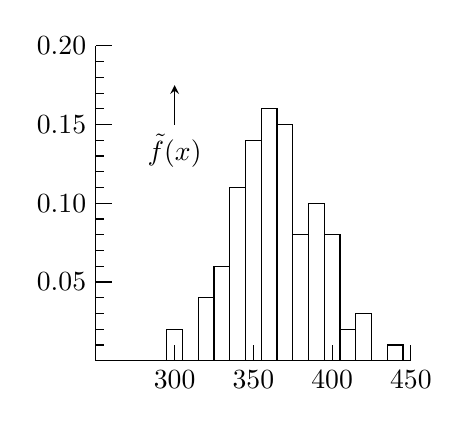
\begin{tikzpicture}
\pgfmathsetmacro{\w}{0.1}
\draw(0,0)--(4,0);
\draw(0,0)--(0,4);
\foreach \y/\ys in {1/0.05,2/0.10,3/0.15,4/0.20}{\draw(0,\y)node[left]{$\ys$}--++(0.2,0);}
\foreach \y in {0.2,0.4,0.6,0.8}{\draw(0,0+\y)--++(0.1,0)  (0,1+\y)--++(0.1,0) (0,2+\y)--++(0.1,0) (0,3+\y)--++(0.1,0);}
\foreach \x/\xs in {1/300,2/350,3/400,4/450}{\draw(\x,0)node[below]{$\xs$}--++(0,0.2);}
\draw(1-\w,0)--++(0,0.4)--++(2*\w,0)--++(0,-0.4);
\draw(1.4-\w,0)--++(0,0.8)--++(2*\w,0);
\draw(1.6-\w,0)--++(0,1.2)--++(2*\w,0);
\draw(1.8-\w,0)--++(0,2.2)--++(2*\w,0);
\draw(2-\w,0)--++(0,2.8)--++(2*\w,0);
\draw(2.2-\w,0)--++(0,3.2)--++(2*\w,0)--++(0,-0.2);
\draw(2.4-\w,0)--++(0,3)--++(2*\w,0)--++(0,-1.4);
\draw(2.6-\w,0)--++(0,1.6)--++(2*\w,0);
\draw(2.8-\w,0)--++(0,2)--++(2*\w,0)--++(0,-0.4);
\draw(3-\w,0)--++(0,1.6)--++(2*\w,0)--++(0,-1.2);
\draw(3.2-\w,0)--++(0,0.4)--++(2*\w,0);
\draw(3.4-\w,0)--++(0,0.6)--++(2*\w,0)--++(0,-0.6);
\draw(3.8-\w,0) rectangle ++(2*\w,0.2);
\draw[-stealth](1,3)node[below]{$\tilde{f}(x)$}--++(0,0.5);
\end{tikzpicture}
\caption*{(پ) تعددی مستطیلی ترسیم}
\end{subfigure}%
\begin{subfigure}{0.5\textwidth}
\centering
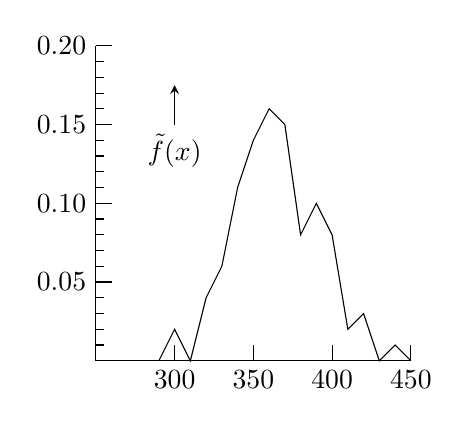
\begin{tikzpicture}
\pgfmathsetmacro{\w}{0.1}
\draw(0,0)--(4,0);
\draw(0,0)--(0,4);
\foreach \y/\ys in {1/0.05,2/0.10,3/0.15,4/0.20}{\draw(0,\y)node[left]{$\ys$}--++(0.2,0);}
\foreach \y in {0.2,0.4,0.6,0.8}{\draw(0,0+\y)--++(0.1,0)  (0,1+\y)--++(0.1,0) (0,2+\y)--++(0.1,0) (0,3+\y)--++(0.1,0);}
\foreach \x/\xs in {1/300,2/350,3/400,4/450}{\draw(\x,0)node[below]{$\xs$}--++(0,0.2);}
\draw(0.8,0)--(1,0.4)--(1.2,0)--(1.4,0.8)--(1.6,1.2)--(1.8,2.2)--(2,2.8)--(2.2,3.2)--(2.4,3)--(2.6,1.6)--(2.8,2)--(3,1.6)--(3.2,0.4)--(3.4,0.6)--(3.6,0)--(3.8,0.2)--(4,0);
\draw[-stealth](1,3)node[below]{$\tilde{f}(x)$}--++(0,0.5);
\end{tikzpicture}
\caption*{(ت) تعددی کثیر الاضلاع ترسیم}
\end{subfigure}%
\caption{ترسیم برائے جدول \حوالہ{جدول_شماریات_تعددی_تقسیم_الف}}
\label{شکل_شماریات_تعددی_ترسیم}
\end{figure}


نمونہ کا \موٹا{ترسیمی اظہار} شکل \حوالہ{شکل_شماریات_تعددی_ترسیم}-الف تا شکل \حوالہ{شکل_شماریات_تعددی_ترسیم}-ت میں دکھایا گیا ہے۔شکل \حوالہ{شکل_شماریات_تعددی_ترسیم}-پ میں ہر مستطیل کا رقبہ مطابقتی اضافی تعدد کے برابر  ہو گا لہٰذا عمودی محدد پر اضافی تعدد فی اکائی رقبہ ہو گا۔چونکہ شکل \حوالہ{شکل_شماریات_تعددی_ترسیم}-پ میں تمام مستطیل کی چوڑائی ایک جیسی ہے  لہٰذا عمودی محدد پر قیمتیں \عددی{\tilde{f}(x)} کے راست متناسب ہوں گی۔ البتہ مستطیل کو چوڑائیاں مختلف ہونے کی صورت میں ایسا نہیں ہو گا۔ شکل \حوالہ{شکل_شماریات_تعددی_ترسیم}-ت میں بھی یہی صورت حال ہو گی۔

ہم اب درج ذیل تفاعل متعارف کرتے ہیں
\begin{align*}
\tilde{F}(x)=\text{\RL{\عددی{x} اور \عددی{x} سے کم تمام قیمتوں کے اضافی تعدد کا مجموعہ}}
\end{align*}
جس کو \اصطلاح{نمونے کا مجموعی  تعددی تفاعل}\فرہنگ{تعددی!نمونے کا مجموعی تفاعل}\حاشیہب{cumulative frequency function of the sample}\فرہنگ{frequency!cumulative function of sample} یا مختصراً \اصطلاح{تقسیمی تفاعل نمونہ}\فرہنگ{تقسیمی تفاعل نمونہ}\فرہنگ{تقسیم!تقسیمی تفاعل نمونہ}\حاشیہب{sample distribution function}\فرہنگ{sample distribution function} کہتے ہیں۔شکل \حوالہ{شکل_شماریات_مجموعی_تعددی_تفاعل} میں مثال دی گئی ہے۔

\begin{figure}
\centering
\begin{subfigure}{1\textwidth}
\centering
\begin{tikzpicture}[x={2cm},y={0.5cm}]
\draw(0,4)--(0,0)--(5,0)node[right]{$x$};
\foreach \y/\ys in {2/0.1,4/0.2}{\draw(0,\y)node[left]{$\ys$}--++(0.2,0);}
\foreach \y in {1,3}{\draw(0,\y)--++(0.1,0);}
\foreach \x/\y in {1/0.2,1.4/0.8,1.6/1.2,1.8/2.2,2/2.8,2.2/3.2,2.4/3,2.6/1.6,2.8/2,3/1.6,3.2/0.4,3.4/0.6,3.8/0.2}{\draw(\x,0)--++(0,\y);}
\draw[-stealth](0.5,3)node[below]{$\tilde{f}(x)$}--++(0,0.5);
\end{tikzpicture}
\end{subfigure}
\begin{subfigure}{1\textwidth}
\centering
\begin{tikzpicture}[x={2cm},y={5cm}]
\draw(0,1)--(0,0)--(5,0)node[right]{$x$};
\foreach \y in {0.2,0.4,0.6,0.8}{\draw(0,0.5*\y)--++(0.1,0)  (0,0.5+0.5*\y)--++(0.1,0);}
\foreach \y in {0.5,1}{\draw(0,\y)node[left]{$\y$}--++(0.2,0);}
\foreach \x/\xs in {1/300,2/350,3/400,4/450}{\draw(\x,0)node[below]{$\xs$}--++(0,0.02);}
\foreach \x in {0.2,0.4,0.6,0.8} {\draw(\x,0)--++(0,0.01) (1+\x,0)--++(0,0.01)  (2+\x,0)--++(0,0.01) (3+\x,0)--++(0,0.01)  (4+\x,0)--++(0,0.01);}
\draw[-stealth](0.5,0.75)node[below]{$\tilde{F}(x)$}--++(0,0.2);
\draw(1,0)--(1,0.02)--(1.4,0.02)--(1.4,0.06)--(1.6,0.06)--(1.6,0.12)--(1.8,0.12)--(1.8,0.23)--(2,0.23)--(2,0.37)--(2.2,0.37)--(2.2,0.53)--(2.4,0.53)--(2.4,0.68)--(2.6,0.68)--(2.6,0.76)--(2.8,0.76)--(2.8,0.86)--(3,0.86)--(3,0.94)--(3.2,0.94)--(3.2,0.99)--(3.8,0.99)--(3.8,1)--(5,1);
\end{tikzpicture}
\end{subfigure}%
\caption{تعددی تفاعل \عددی{\tilde{f}(x)} اور مجموعی تعددی تفاعل \عددی{\tilde{F}(x)} برائے جدول \حوالہ{جدول_شماریات_تعددی_تقسیم_الف}}
\label{شکل_شماریات_مجموعی_تعددی_تفاعل}
\end{figure}

\عددی{\tilde{F}(x)} \ترچھا{سیڑھی تفاعل} (ٹکڑوں میں مستقل تفاعل) ہے جس میں ٹھیک ان \عددی{x}  پر جہاں \عددی{\tilde{f}(x)\ne0} ہو \عددی{\tilde{f}(x)} کے برابر چلانگ پائے جاتے ہیں۔پہلی چھلانگ نمونہ کی کم سے کم قیمت اور آخری چھلانگ نمونہ کی زیادہ سے زیادہ قیمت پر پائی جائے گی۔ آخری چھلانگ  کے بعد \عددی{\tilde{F}(x)=1} رہے گا۔

\عددی{\tilde{f}(x)} اور \عددی{\tilde{F}(x)} کا تعلق درج ذیل ہے
\begin{align}
\tilde{F}(x)=\sum_{t\le x}\tilde{f}(t)
\end{align}
جہاں \عددی{t\le x} کا مطلب  ہے کہ کسی بھی \عددی{x} کے لئے ان تمام \عددی{\tilde{f}(x)} کا مجموعہ لیا جائے گا جن کے لئے \عددی{t} کی قیمت \عددی{x} کے برابر یا \عددی{x} سے کم ہو۔

اگر کسی نمونہ میں مختلف اعداد کی تعداد بہت زیادہ ہو تب اس کا جدولی اور ترسیمی  اظہار غیر ضروری طور پر مشکل ہو گا جس کو \اصطلاح{گروہ بندی}\فرہنگ{گروہ بندی}\حاشیہب{grouping}\فرہنگ{grouping} سے آسان بنانا ممکن ہے۔آئیں گروہ بندی کے عمل کو سمجھیں۔

دیے گئے نمونہ کے لحاظ سے ہم ایسا وقفہ \عددی{I} منتخب کرتے ہیں جس میں تمام نمونی  قیمتیں شامل ہوں۔ہم \عددی{I} کو ٹکڑوں میں تقسیم کرتے ہیں جنہیں \اصطلاح{جماعتی وقفہ}\فرہنگ{جماعتی!وقفہ}\حاشیہب{class intervals}\فرہنگ{class!intervals} کہتے ہیں۔ان جماعتی وقفوں کے وسطی نقطوں کو \اصطلاح{جماعتی وسطی نقطے}\فرہنگ{جماعتی_وسطی نقطہ}\حاشیہب{class midpoints}\فرہنگ{class!midpoints} یا \اصطلاح{جماعتی نشان}\فرہنگ{جماعتی!نشان}\حاشیہب{class marks}\فرہنگ{class!marks} کہتے ہیں۔ہر جماعتی وقفہ میں پائے جانے والے نمونی قیمتیں کو \اصطلاح{طبقہ}\فرہنگ{طبقہ}\حاشیہب{class}\فرہنگ{class} کہتے ہیں۔ طبقہ  میں نمونی قیمتوں کی تعداد کو \اصطلاح{جماعتی تعدد}\فرہنگ{جماعتی!تعدد}\حاشیہب{class frequency}\فرہنگ{class!frequency} کہتے ہیں جس کو جسامت نمونہ \عددی{n} سے تقسیم کرنے سے \اصطلاح{اضافی جماعتی تعدد}\فرہنگ{جماعتی!اضافی تعدد}\حاشیہب{relative class frequency}\فرہنگ{class!relative frequency} حاصل ہو گا۔ اس تعدد \عددی{\tilde{f}(x)} کو جو جماعتی نشان کے تابع ہے  \اصطلاح{گروہ بند نمونہ کا تعددی تفاعل}\فرہنگ{تعددی! تفاعل، گروہ بند نمونہ}\حاشیہب{frequency function of the grouped sample}\فرہنگ{frequency!function of the grouped sample} کہتے ہیں۔اسی طرح  مجموعی اضافی جماعتی تعدد \عددی{\tilde{F}(x)} جو جماعتی نشان کے تابع ہے \اصطلاح{گروہ بند نمونہ کا تقسیمی تفاعل}\فرہنگ{تقسیمی!تفاعل،گروہ بند نمونہ}\فرہنگ{distribution function of the grouped sample}\حاشیہب{distribution!function of the grouped sample} کہلاتا ہے۔جدول \حوالہ{جدول_شماریات_دھاگہ_مضبوطی} اور جدول \حوالہ{جدول_شماریات_تعددی_گروہ_بند} میں مثال دیا گیا ہے۔
\begin{table}
\caption{کپاس کے سوتی دھاگے کو توڑنے کے لئے درکار قوت (نیوٹن میں)}
\label{جدول_شماریات_دھاگہ_مضبوطی}
\centering
\begin{otherlanguage}{english}
\begin{tabular}{RRRRRRRRRR}
\hline
114&118&86&107&87&94&82&81&98&84\\
120&126&98&89&114&83&94&106&96&111\\
123&110&83&118&83&96&96&74&91&81\\
102&107&103&80&109&71&96&91&86&129\\
130&104&86&121&96&96&127&94&102&87\\
\hline
\end{tabular}
\end{otherlanguage}
\end{table}

\begin{table}
\caption{تعددی جدول برائے جدول \حوالہ{جدول_شماریات_دھاگہ_مضبوطی} (گروہ بند)}
\label{جدول_شماریات_تعددی_گروہ_بند}
\centering
\begin{otherlanguage}{english}
\begin{tabular}{R|C|L|R|R|R}
\hline
\multirow{2}{*}{\text{\RL{\urdufont{جماعتی وقفہ}}}}&\text{\RL{\urdufont{جماعتی نشان}}}&\multicolumn{2}{C|}{\text{\RL{\urdufont{حتمی تعدد}}}}&\multirow{2}{*}{$\tilde{f}(x)$}&\multirow{2}{*}{$\tilde{F}(x)$}\\
\cline{3-4}
&x&\text{\RL{\urdufont{نشان شمار}}}&&&\\
\hline
65- 75&70&||&2&0.04&0.04\\
75- 85&80&&8&0.16&0.20\\
85- 95&90&&11&0.22&0.42\\
95-105&100&&12&0.24&0.66\\
105-115&110&&8&0.16&0.82\\
115-125&120&&5&0.10&0.92\\
125-135&130&&4&0.08&1.00\\
\hline
&&\text{\urdufont{مجموعہ}}&50&1.00&\\
\hline
\end{tabular}
\end{otherlanguage}
\end{table}

جماعتوں کی تعداد جتنی کم رکھی جائے، گروہ بند نمونہ کی تقسیم اتنی  سادہ ہو گی اور اتنی ہی زیادہ معلومات کھوئی جائے گی چونکہ اصل نمونی قیمتیں اب صریحاً نظر نہیں آئیں گی۔گروہ بندی کرتے وقت دھیان رکھیں کہ صرف غیر ضروری معلومات کھوئی جائے۔ گروہ بند نمونہ استعمال کرتے ہوئے مشکلات سے بچنے کی خاطر درج ذیل اصولوں کا خیال رکھیں۔
\begin{itemize}
\item
جماعتی وقفے برابر رکھیں۔
\item
جماعتی نشان یوں منتخب کریں کہ جماعتی نشان سادہ اعداد (جن میں غیر صفر ہندسوں کی تعداد کم سے کم ہو) پر واقع ہوں۔
\item
اگر نمونی قیمت \عددی{x_j} دو جماعتوں کی سرحد پر واقع ہو تب یہ قیمت اس طبقہ میں شامل کیا جائے گا جو \عددی{x_j} سے شروع ہوتا ہو۔ 
\end{itemize}

%==========================
\حصہء{سوالات}
%==============
سوال \حوالہ{سوال_شماریات_ترسیم_الف} تا سوال \حوالہ{سوال_شماریات_ترسیم_ب} میں دیے گئے نمونہ کا تعددی جدول بنائیں اور نمونہ کو تعددی نقطہ ترسیم، ڈبہ ترسیم اور مستطیل ترسیم کی صورت میں دکھائیں۔

%==================
\ابتدا{سوال}\شناخت{سوال_شماریات_ترسیم_الف}\quad مزاحمت کی قیمت اوہم \عددی{\si{\ohm}} میں۔
\begin{align*}
\begin{array}{rrrrrrrrrr}
99&100&102&101&98&103&100&102&99&101\\
100&100&99&101&100&102&99&101&98&100
\end{array}
\end{align*}

\انتہا{سوال}
%====================
\ابتدا{سوال}\شناخت{سوال_شماریات_درکار_ترسیم_ت}\quad 
\begin{align*}
\begin{array}{rrrrrrrrrrrrrrr}
6& 2& 4& 1& 2& 4& 3& 3& 2& 1& 6& 5& 6& 3& 4
\end{array}
\end{align*}

\انتہا{سوال}
%========================
\ابتدا{سوال}\شناخت{سوال_شماریات_ترسیم_پ}\quad برقی سوئچ کا سیکنڈوں میں دورانیہ ردعمل 
\begin{align*}
\begin{array}{rrrrrrrrrr}
1.3&1.4&1.1&1.5&1.4&1.3&1.2&1.4&1.5&1.3\\
1.2&1.3&1.5&1.4&1.4&1.6&1.3&1.5&1.1&1.4
\end{array}
\end{align*}
\انتہا{سوال}
%=============================
\ابتدا{سوال}\شناخت{سوال_شماریات_درکار_ترسیم_ٹ}\quad خام کوئلہ میں کوئلہ کی فی صد مقدار
\begin{align*}
\begin{array}{rrrrrrrrrr}
87&86&85&87&86&87&86&81&77&85\\
86&84&83&83&82&84&83&79&82&73
\end{array}
\end{align*}
\انتہا{سوال}
%=============================
\ابتدا{سوال}\quad چادری فولاد کی تنشی مضبوطی [\si{\kilo\gram\per\milli\meter\squared}]
\begin{align*}
\begin{array}{rrrrrrrrrrrrrrr}
44&43&41&41&44&44&43&44&42&45&43&43&44&45&46\\
42&45&41&44&44&43&44&46&41&43&45&45&42&44&44
\end{array}
\end{align*}
\انتہا{سوال}
%=============================
\ابتدا{سوال}\quad  خود کار نظام سے \عددی{100} کاغذ  کے گھٹے بنانے میں کمی بیشی
\begin{align*}
\begin{array}{rrrrrrrrrr}
0&-1&0&0&1&1&2&0&1&0
\end{array}
\end{align*}
\انتہا{سوال}
%=============================
\ابتدا{سوال}\quad  ایک ہی قسم کے گاڑیوں کا تیل کا خرچہ۔  [کلومیٹر فی لیٹر]  
\begin{align*}
\begin{array}{rrrrrr}
12& 11.5&11&12.5&11&12
\end{array}
\end{align*}
\انتہا{سوال}
%=============================
\ابتدا{سوال}\quad  خود کار نظام سے بھری گئی تھیلوں کا گرام میں وزن
\begin{align*}
\begin{array}{rrrrrrrr}
200&203&199&198&201&200&201&201
\end{array}
\end{align*}
\انتہا{سوال}
%=============================
\ابتدا{سوال}\شناخت{سوال_شماریات_ترسیم_ب}\quad  اندرون شہر چلتی ریل گاڑی کا اڈے پر ٹھیک وقت پر پہنچنے سے انحراف (منٹوں میں)\حاشیہد{امید کی جا سکتی ہے کہ ایک دن ہماری ریل گاڑیاں بھی وقت کی اتنی پابند ہوں گی۔}
\begin{align*}
\begin{array}{rrrrrrrrrr}
3&4&1&0&2&2&3&1&5&3
\end{array}
\end{align*}
\انتہا{سوال}
%=============================
\ابتدا{سوال}\شناخت{سوال_شماریات_درکار_الف}\quad
سوال \حوالہ{سوال_شماریات_ترسیم_پ} کے نمونہ کی مجموعی تعددی تفاعل کا ترسیم کھینچیں۔
\انتہا{سوال}
%===========================
\ابتدا{سوال}\quad
جدول \حوالہ{جدول_شماریات_تعددی_گروہ_بند} کے گروہ بند نمونہ کا ڈبہ ترسیم، مستطیل ترسیم اور تعددی کثیر الاضلاع ترسیم کھینچیں۔ 
\انتہا{سوال}
%======================
\ابتدا{سوال}\quad
جدول \حوالہ{جدول_شماریات_کنکریٹ_بیلن} میں جماعتی وقفوں کے جماعتی نشان \عددی{300}، \عددی{320}، \عددی{340}، \نقطے پر لیتے ہوئے مطابقتی تعددی جدول بنائیں۔اس کے مستطیل ترسیم کھینچ کا شکل \حوالہ{شکل_شماریات_تعددی_ترسیم}-پ کے ساتھ موازنہ کریں۔
\انتہا{سوال}
%===========================
\ابتدا{سوال}\quad
جدول \حوالہ{جدول_شماریات_دھاگہ_مضبوطی} میں جماعتی نشان \عددی{75}، \عددی{85}، \عددی{95}، \نقطے لے کر مطابقتی تعددی جدول بنائیں۔اس کے مستطیل ترسیم کا سوال \حوالہ{سوال_شماریات_درکار_الف} کے ترسیم سے موازنہ کریں۔  
\انتہا{سوال}
%===================
\ابتدا{سوال}\quad
\عددی{1500} تجرباتی نتائج میں سب سے کم ناپ \عددی{\SI{10.8}{\centi\meter}} اور سب سے زیادہ ناپ \عددی{\SI{11.9}{\centi\meter}} تھی۔اس مواد کی گروہ بندی لے لئے جماعتی وقفہ تجویز کریں۔
\انتہا{سوال}
%==================

\حصہ{نمونی اوسط اور نمونی تغیریت}
تعددی تفاعل (یا تقسیمی تفاعل) نمونہ کی صحیح تصویر کشی کرتا ہے۔اس تفاعل سے ہم نمونہ کے کئی خواص کا حساب لگا سکتے ہیں مثلاً نمونی قیمتوں کی اوسط جسامت، پھیل، تشاکل، وغیرہ۔ اس حصہ میں ہم ایسے اہم ترین دو قیمتوں، نمونی اوسط اور نمونی تغیریت، پر غور کریں گے۔

نمونہ \عددی{x_1,x_2,\cdots,x_n} کی اوسط قیمت یا مختصراً \اصطلاح{نمونی اوسط}\فرہنگ{نمونی!اوسط}\فرہنگ{اوسط}\حاشیہب{sample mean}\فرہنگ{sample!mean} کو \عددی{\bar{x}} سے ظاہر کیا جاتا ہے جس کی تعریف درج ذیل کلیہ دیتی ہے۔
\begin{align}\label{مساوات_شماریات_نمونی_اوسط_الف}
\bar{x}=\frac{1}{n}\sum_{j=1}^{n}x_j=\frac{1}{n}(x_1+x_2+\cdots+x_n)
\end{align}
تمام نمونی قیمتوں کے مجموعہ کو جسامت \عددی{n} سے تقسیم کرتے ہوئے نمونی اوسط حاصل ہو گا۔ظاہر ہے کہ یہ نمونی قیمتوں کی اوسط جسامت دے گا۔

نمونہ \عددی{x_1,x_2,\cdots,x_n} کی \اصطلاح{نمونی تغیریت}\فرہنگ{نمونی!تغیریت}\فرہنگ{تغیریت}\حاشیہب{sample variance}\فرہنگ{sample!variance} کو \عددی{s^2} سے ظاہر کیا جاتا ہے جس کی تعریف درج ذیل کلیہ دیتی ہے۔
\begin{gather}
\begin{aligned}\label{مساوات_شماریات_نمونی_اوسط_ب}
s^2&=\frac{1}{n-1}\sum_{j=1}^{n}(x_j-\bar{x})^2\\
&=\frac{1}{n-1}[(x_1-\bar{x})^2+(x_2-\bar{x})^2+\cdots +(x_n-\bar{x})^2]
\end{aligned}
\end{gather}
نمونی اوسط \عددی{\bar{x}} سے نمونی قیمتوں کے انحراف کے مربعوں کو \عددی{n-1} سے تقسیم کرتے ہوئے نمونی تغیریت حاصل ہو گی۔یہ نمونی قیمتوں کی انحراف یا پھیل کی ناپ ہے۔نمونی تغیریت غیر منفی عدد ہو گا۔ نمونی تغیریت \عددی{s^2} کا مثبت جذر \اصطلاح{معیاری انحراف}\فرہنگ{معیاری انحراف}\حاشیہب{standard deviation}\فرہنگ{standard deviation} کہلاتا ہے جس کو \عددی{s} سے ظاہر کیا جاتا ہے۔

%=================
\ابتدا{مثال}\شناخت{مثال_شماریات_اوسط}\quad \موٹا{نمونی اوسط اور نمونی تغیریت}\\
بے ترتیب منتخب کیے گئے کیلوں کی  (سنٹی میٹروں میں) لمبائیاں درج ذیل ہیں۔
\begin{align*}
\begin{array}{cccccccccc}
0.80&0.81&0.81&0.82&0.81&0.82&0.80&0.82&0.81&0.81
\end{array}
\end{align*}
مساوات \حوالہ{مساوات_شماریات_نمونی_اوسط_الف} سے نمونی اوسط
\begin{align*}
\bar{x}=\frac{1}{10}(0.80+0.81+0.81+0.82+\cdots+0.81)=\SI{0.811}{\centi\meter}
\end{align*}
اور مساوات \حوالہ{مساوات_شماریات_نمونی_اوسط_ب} سے نمونی تغیریت
\begin{align*}
s^2=\frac{1}{9}[(0.80-0.811)^2+\cdots+(0.81-0.811)^2]=\SI{0.000054}{\centi\meter\squared}
\end{align*}
ہے۔ایک جیسی نمونی قیمتوں کو اکٹھا لکھنے سے حساب نسبتاً آسان بنایا جا سکتا ہے جیسے
\begin{align*}
\bar{x}=\frac{1}{10}(2\cdot 0.80+5\cdot 0.81+3\cdot 0.82)=\SI{0.811}{\centi\meter}
\end{align*} 
جہاں قوسین میں تین مختلف نمونی قیمتوں \عددی{x_1=0.80}، \عددی{x_2=0.81} اور \عددی{x_3=0.82} کو ان کی تعدد سے ضرب دیا گیا ہے۔اسی طرح
\begin{align*}
s^2=\frac{1}{9}[(2(0.800-0.811)^2+5(0.810-0.811)^2+3(0.820-0.811)^2]=\num{0.000054}
\end{align*}
ہو گا۔
\انتہا{مثال}
%=========================
اس مثال میں ہم نے \عددی{\bar{x}} اور \عددی{s^2} کو نمونہ کے تعددی تفاعل \عددی{\tilde{f}(x)} کی مدد سے حاصل کرنا دیکھا۔اگر ایک نمونہ میں ٹھیک \عددی{m} مختلف اعدادی قیمتیں 
\begin{align*}
x_1, x_2,\cdots, x_m
\end{align*}
پائی جاتی ہوں جن کے مطابقتی اضافی تعدد
\begin{align*}
\tilde{f}(x_1),\tilde{f}(x_2),\cdots,\tilde{f}(x_m)
\end{align*}
ہوں تب حساب کے لئے درکار تعدد درج ذیل ہوں گے
\begin{align*}
n\tilde{f}(x_1),n\tilde{f}(x_2),\cdots,n\tilde{f}(x_m)
\end{align*}
جنہیں استعمال کرتے ہوئے مساوات \حوالہ{مساوات_شماریات_نمونی_اوسط_الف} اور مساوات \حوالہ{مساوات_شماریات_نمونی_اوسط_ب} سے
\begin{align}\label{مساوات_شماریات_نمونی_اوسط_پ}
\bar{x}=\frac{1}{n}\sum_{j=1}^{m}x_jn\tilde{f}(x_j)
\end{align}
اور
\begin{align}\label{مساوات_شماریات_نمونی_اوسط_ت}
s^2=\frac{1}{n-1}\sum_{j=1}^{m} (x_j-\bar{x})^2n\tilde{f}(x_j)
\end{align}
حاصل ہو گا۔ دھیان رہے کہ مساوات \حوالہ{مساوات_شماریات_نمونی_اوسط_الف} اور مساوات \حوالہ{مساوات_شماریات_نمونی_اوسط_ب} میں ہم تمام نمونی قیمتوں پر مجموعہ لیتے ہیں جبکہ مساوات \حوالہ{مساوات_شماریات_نمونی_اوسط_پ} اور مساوات \حوالہ{مساوات_شماریات_نمونی_اوسط_ت} میں ہم اعدادی طور مختلف نمونی قیمتوں پر مجموعہ حاصل کرتے ہیں۔حتمی تعدد \عددی{n\tilde{f}(x_j)} عدد صحیح ہوں گے جبکہ اضافی تعدد \عددی{\tilde{f}(x_j)} عموماً غیر عدد صحیح ہوں گے۔

چونکہ \عددی{x_j-\bar{x}} کی حتمی قیمت نمونی اوسط کی نسبت بہت کم ہو سکتی ہے لہٰذا \عددی{s^2} کے مذکورہ بالا کلیات کی استعمال سے (خود کار حساب میں) ملحوظ ہندسے ضائع ہوں گے۔ہم \عددی{s^2} کا ایک ایسا کلیہ اخذ کرتے ہیں جو ان مشکلات سے دو چار نہ ہو۔ہم  مساوات \حوالہ{مساوات_شماریات_نمونی_اوسط_ب} میں
\begin{align*}
(x_j-\bar{x})^2=x_j^2-2x_j\bar{x}+\bar{x}^2
\end{align*}
پر کرتے ہوئے تین مجموعے 
\begin{align*}
\sum(x_j-\bar{x})^2=\sum x_j^2-2\bar{x}\sum x_j+\sum \bar{x}^2
\end{align*}
حاصل کرتے ہیں جہاں آخری مجموعہ \عددی{n\bar{x}^2} کے برابر ہے۔ مساوات \حوالہ{مساوات_شماریات_نمونی_اوسط_الف} سے \عددی{\bar{x}} کی قیمت پر کرتے ہوئے
\begin{align*}
-2\bar{x}\sum x_j=-\frac{2}{n}(\sum x_j)^2 \quad \text{اور}\quad n\bar{x}^2=\frac{1}{n}(\sum x_j)^2
\end{align*}
لکھا جا سکتا ہے جنہیں استعمال کرتے ہوئے
\begin{align}\label{مساوات_شماریات_نمونی_اوسط_ٹ}
s^2=\frac{1}{n-1}\big[\sum_{j=1}^{n}x_j^2-\frac{1}{n}\big(\sum_{j=1}^{n}x_j\big)^2\big]
\end{align}
حاصل ہو گا۔ اسی طرح  مساوات \حوالہ{مساوات_شماریات_نمونی_اوسط_ت} کو تبدیل کرتے ہوئے
\begin{align}\label{مساوات_شماریات_نمونی_اوسط_ث}
s^2=\frac{1}{n-1}\big[\sum_{j=1}^{m} x_j^2n\tilde{f}(x_j)-\frac{1}{n}\big(\sum_{j=1}^{m}x_jn\tilde{f}(x_j)\big)^2\big]
\end{align}
حاصل کیا جا سکتا ہے۔

مثال کے طور پر مثال \حوالہ{مثال_شماریات_اوسط} میں مساوات \حوالہ{مساوات_شماریات_نمونی_اوسط_پ} اور مساوات \حوالہ{مساوات_شماریات_نمونی_اوسط_ث} (جدول \حوالہ{جدول_شماریات_اوسط_تغیریت}) سے پہلے کی طرح \عددی{\bar{x}=\tfrac{8.11}{10}=0.811} اور  
\begin{align*}
s^2=\frac{1}{9}\big(6.5777-\frac{8.11^2}{10}\big)=\frac{\num{0.00049}}{9}=\num{0.000054}
\end{align*}
حاصل ہوتے ہیں۔
\begin{table}
\caption{اوسط اور تغیریت کا حساب برائے مثال \حوالہ{مثال_شماریات_اوسط}}
\label{جدول_شماریات_اوسط_تغیریت}
\centering
\begin{otherlanguage}{english}
\begin{tabular}{C|C|C|C|C}
\hline
\Tstrut
x_j&10\tilde{f}(x_j)&x_j\cdot 10 \tilde{f}(x_j)&x_j^2&x_j^2\cdot 10 \tilde{f}(x_j)\\
\hline
0.80&2&1.60&0.6400&1.2800\\
0.81&5&4.05&0.6561&3.2805\\
0.82&3&2.46&0.6724&2.0172\\
\hline
\end{tabular}
\end{otherlanguage}
\end{table}

%=======================
\حصہء{سوالات}
%=====================
\ابتدا{سوال}\quad
گزشتہ حصے کی سوال \حوالہ{سوال_شماریات_درکار_ترسیم_ت} کے لئے نمونی اوسط اور نمونی تغیریت تلاش کریں۔\\
جواب:\quad
$\bar{x}=3.47,\,\, s^2=2.98$
\انتہا{سوال}
%=======================
\ابتدا{سوال}\quad
گزشتہ حصے کی سوال \حوالہ{سوال_شماریات_درکار_ترسیم_ٹ} کے لئے نمونی اوسط اور نمونی تغیریت تلاش کریں۔\\
جواب:\quad
$\bar{x}=84,\,\,s^2=\tfrac{1251}{95}$
\انتہا{سوال}
%=======================
\ابتدا{سوال}\quad
نمونہ \عددی{2,1,4,5} کا مستطیل ترسیم کھینچیں۔ترسیم کو دیکھ کر \عددی{\bar{x}} اور \عددی{s} کی قیمتوں کا اندازہ لگائیں۔\عددی{\bar{x}}، \عددی{s^2} اور \عددی{s} کی قیمتوں کا حساب لگائیں۔\\
جواب:\quad
$\bar{x}=3,\,\, s^2=3.3,\,\, s=1.817$
\انتہا{سوال}
%=====================
\ابتدا{سوال}\quad
دکھائیں کہ کم سے کم اور زیادہ سے زیادہ نمونی قیمتوں کے بیچ \عددی{\bar{x}} ہو گا۔
\انتہا{سوال}
%===========================
\ابتدا{سوال}\quad \موٹا{نمونہ کی سعت}\\
نمونہ میں سب سے بڑی قیمت اور سب سے چھوٹی قیمت کے فرق کو نمونہ کی \اصطلاح{سعت}\فرہنگ{سعت}\حاشیہب{range}\فرہنگ{range} کہتے ہیں۔مثال \حوالہ{مثال_شماریات_اوسط} میں دیے گئے نمونہ کی سعت تلاش کریں۔\\
جواب:\quad
$0.02$
\انتہا{سوال}
%==========================
\ابتدا{سوال}\quad \موٹا{صدویہ، وسطانیہ}\\
نمونہ کی \عددی{p} ویں \اصطلاح{صدویہ}\فرہنگ{صدویہ}\حاشیہب{percentile}\فرہنگ{percentile} سے مراد ایسا عدد \عددی{Q_p} ہے کہ کم از کم \عددی{p\,\si{\percent}} نمونی قیمتیں \عددی{Q_p} سے کم یا اس کے برابر ہوں اور ساتھ ہی \عددی{(100-p)\,\si{\percent}} نمونی قیمتیں اس سے زیادہ یا اس کے برابر ہوں۔اگر ایک سے زیادہ ایسا عدد پایا جاتا ہو (جس صورت میں ان اعداد کا وقفہ پایا جائے گا) تب \عددی{p} ویں صدویہ سے مراد ان اعداد کا اوسط (یعنی وقفے  کا وسطی نقطہ) ہو گا۔بالخصوص \عددی{Q_{50}} کو \اصطلاح{وسطانیہ}\فرہنگ{وسطانیہ}\حاشیہب{median}\فرہنگ{median} کہتے ہیں جس کو \عددی{\tilde{x}} سے ظاہر کیا جاتا ہے۔وسطانیہ کو \اصطلاح{نصف چوتھائی}\فرہنگ{چوتھائی!نصف}\حاشیہب{middle quartile}\فرہنگ{quartile!middle} بھی کہتے ہیں۔جدول \حوالہ{جدول_شماریات_تعددی_تقسیم_الف} کے نمونہ  کا وسطانیہ \عددی{\tilde{x}} تلاش کریں۔\\
جواب:\quad
$360$
\انتہا{سوال}
%==========================
\ابتدا{سوال}\شناخت{سوال_شماریات_چوتھائی_الف}\quad 
نمونہ کی \عددی{Q_{25}} اور \عددی{Q_{75}} صدویہ کو بالترتیب \اصطلاح{نچلی چوتھائی}\فرہنگ{چوتھائی!نچلی}\حاشیہب{lower quartile}\فرہنگ{quartile!lower} اور \اصطلاح{بالائی چوتھائی}\فرہنگ{چوتھائی!بالائی}\حاشیہب{upper quartile}\فرہنگ{quartile!upper} کہتے ہیں جبکہ \عددی{Q_{75}-Q_{25}} جو پھیل کی ناپ ہے کو \اصطلاح{چوتھائی سعت}\فرہنگ{چوتھائی!سعت}\حاشیہب{interquartile range}\فرہنگ{quartile!interquartile range} کہتے ہیں۔جدول \حوالہ{جدول_شماریات_تعددی_تقسیم_الف} کے نمونہ  کا کی \عددی{Q_{25}}، \عددی{Q_{75}} اور \عددی{Q_{75}-Q_{25}} تلاش کریں۔\\
جواب:\quad
$350,\,\,380,\,\,30$
\انتہا{سوال}
%=============================
\ابتدا{سوال}\quad
جدول \حوالہ{جدول_شماریات_دھاگہ_مضبوطی} کے لئے سوال \حوالہ{سوال_شماریات_چوتھائی_الف} کو حل کریں۔\\
جواب:\quad
$\tfrac{345}{4},\,\,\tfrac{439}{4},\,\,\tfrac{47}{2}$
\انتہا{سوال}
%=========================
\ابتدا{سوال}\quad \موٹا{عادہ}\\
نمونہ میں سب سے زیادہ بار آنے والی قیمت کو نمونہ کی \اصطلاح{عادہ}\فرہنگ{عادہ}\حاشیہب{mode}\فرہنگ{mode} کہتے ہیں۔یہ سب سے عام قدر ہوتی ہے۔درج ذیل نمونہ کی اوسط، وسطانیہ اور عادہ تلاش کریں۔ ان پر تبصرہ کریں۔
\begin{align*}
\begin{array}{L|CCC}
\text{\RL{\urdufont{قیمت}}}&100&1000&\num{1000000}\\
\hline
\text{\RL{\urdufont{تعدد}}}&100&90&20
\end{array}
\end{align*}
جواب:\quad
$\text{اوسط}=\num{10000},\,\, \text{وسطانیہ}=1000,\,\,\text{عادہ}=100$
\انتہا{سوال}
%===========================
\ابتدا{سوال}\شناخت{سوال_شماریات_مبدا_کام}\quad \موٹا{مبدا کام}\\
اگر \عددی{x_j=x^*_j+c} ہو جہاں  \عددی{j=1,\cdots,n} اور \عددی{c} کوئی مستقل ہو تب دکھائیں کہ
\begin{align*}
\bar{x}=c+\bar{x}^*,\quad \big(\bar{x}^*=\frac{1}{n}\sum_{j=1}^{n}x_j^*\big)\quad  \text{اور} \quad \quad s^2=s^{*2}
\end{align*}
ہوں گے جہاں \عددی{x_j^*} قیمتوں  کی تغیریت \عددی{s^{*2}} ہے۔(عملی استعمال میں \عددی{c} یوں منتخب کیا جاتا ہے کہ \عددی{x_j^*} کی حتمی قیمتیں چھوٹی ہوں۔جیومیٹریائی طور پر یہ مبدا کی تبدیلی کے مترادف ہے لہٰذا اس کو \ترچھا{ترکیب مبدا کام}\فرہنگ{ترکیب!مبدا کام}\حاشیہب{method of working origin}\فرہنگ{method!of working origin} کہتے ہیں۔)  
\انتہا{سوال}
%=========================
\ابتدا{سوال}\quad
ترکیب مبدا کام کو مثال \حوالہ{مثال_شماریات_اوسط} کے نمونہ پر لاگو کریں۔
\انتہا{سوال}
%====================
\ابتدا{سوال}\quad \موٹا{مکمل رمز نویسی}\\
اگر \عددی{x_j=c_1x_j^*+c_2} ہو جہاں \عددی{j=1,\cdots,n} جبکہ \عددی{c_1} اور \عددی{c_2} مستقل ہیں تب دکھائیں کہ
\begin{align*}
\bar{x}=c_1\bar{x}^*+c_2,\quad s^2=c_1^2s^{*2}
\end{align*}
ہوں گے جہاں \عددی{\bar{x}^*} اور \عددی{s^{*2}} کی معنی سوال \حوالہ{سوال_شماریات_مبدا_کام} میں پیش کی گئی ہیں۔اس کو \اصطلاح{ترکیب مکمل رمز نویسی}\فرہنگ{ترکیب!مکمل رمز نویسی}\حاشیہب{method of full coding}\فرہنگ{method!of full coding} کہتے ہیں۔(اس ترکیب سے قلم و کاغذ استعمال کرتے ہوئے نتائج کی جلد جانچ پڑتال کی جا سکتی ہے۔)
\انتہا{سوال}
%======================
\ابتدا{سوال}\quad
اس ترکیب کو مثال \حوالہ{مثال_شماریات_اوسط} کے نمونہ پر لاگو کریں۔
\انتہا{سوال}
%======================
\ابتدا{سوال}\quad
کسی بھی نمونہ کی گروہ بندی سے عموماً نمونی اوسط متاثر ہو گا۔دکھائیں کہ نمونی اوسط میں تبدیل \عددی{\tfrac{l}{2}} سے زیادہ نہیں ہو سکتی ہے جہاں ہر ایک جماعتی وقفہ کی لمبائی \عددی{l} ہے۔
\انتہا{سوال}
%=======================
\ابتدا{سوال}\quad
جدول \حوالہ{جدول_شماریات_دھاگہ_مضبوطی} کی غیر گروہ بند نمونہ کی گروہ بندی  جدول \حوالہ{جدول_شماریات_تعددی_گروہ_بند} میں کی گئی ہے۔دونوں مواد کی اوسط اور تغیریت تلاش کریں۔نتائج کا آپس میں موازنہ کریں۔\\
جواب:\quad
$\text{غیر گروہ بند}:\,\, \bar{x}=99.2,\,\, s^2=234.7;\quad \text{گروہ بند}:\,\, \bar{x}=99.4,\,\, s^2=254.7$
\انتہا{سوال}
%===========================

\حصہ{بے قاعدہ تجربات، نتائج،}
شماریاتی تجربات یا شماریاتی مشاہدے  سے ہمیں نمونے حاصل ہوں گے جن کی مدد سے ہم مطابقتی  آبادی کے بارے میں نتائج اخذ کرنا چاہیں گے۔ایسا کرنے سے پہلے  حسابی امکانیات کی مدد سے ہمیں آبادی کے حسابی نمونے  بنانے ہوں گے۔یہ نظریہ حسابی شماریات کی بنیاد ہے جس کی گہرائی میں ہم اپنی ضرورت کے مطابق  جائیں گے۔اس حصہ میں کئی بنیادی تصورات کو متعارف کیا جائے گا۔

ایک بے قاعدہ تجربہ یا بے قاعدہ مشاہدہ، جنہیں ہم مختصراً \اصطلاح{تجربہ}\فرہنگ{تجربہ}\حاشیہب{experiment}\فرہنگ{experiment} یا \اصطلاح{مشاہدہ}\فرہنگ{مشاہدہ}\حاشیہب{observation}\فرہنگ{observation} کہیں گے، سے مراد وہ عمل ہے جو درج ذیل خواص رکھتا ہو۔
\begin{itemize}
\item
اس کو طے شدہ قواعد کے تحت سرانجام دیا جاتا ہے جو عمل کو مکمل طور پر بیان کرتے ہیں۔
\item
اس  عمل کو جتنی بار چاہیں دوبارہ انجام  دیا جا سکتا ہے۔
\item
ہر مرتبہ عمل کا نتیجہ  اتفاق پر منحصر ہو گا (یعنی نتیجہ ان اثرات پر منحصر ہے جنہیں ہم قابو نہیں کر سکتے ہیں) لہٰذا قبل از وقت  یکتا طور پر نتیجہ جاننا ممکن نہیں ہو گا۔
\end{itemize} 

ایک مرتبہ تجربے کے عمل سے حاصل نتیجہ کو \اصطلاح{کوشش}\فرہنگ{کوشش}\حاشیہب{trial}\فرہنگ{trial} کا \اصطلاح{انجام}\فرہنگ{انجام}\حاشیہب{outcome}\فرہنگ{outcome} کہا جاتا ہے۔
